
\chapter{Implementation}

\section{Operation}
Operation are used to decribe changements made in a document. For this purpose they must contain the information: \emph{what} has to be changed and \emph{where} this has to be changed.

In case of simple text editing only two operations are required. An insert operation (e.g. \texttt{Ins(1,'hello')}) which will insert the string 'hello' at position 1 and an delete operation (e.g. \texttt{Del(10, 'world')}) which will delete the string 'world' at position 10. With this two operation all can be made.

\begin{figure}[H]
\centering
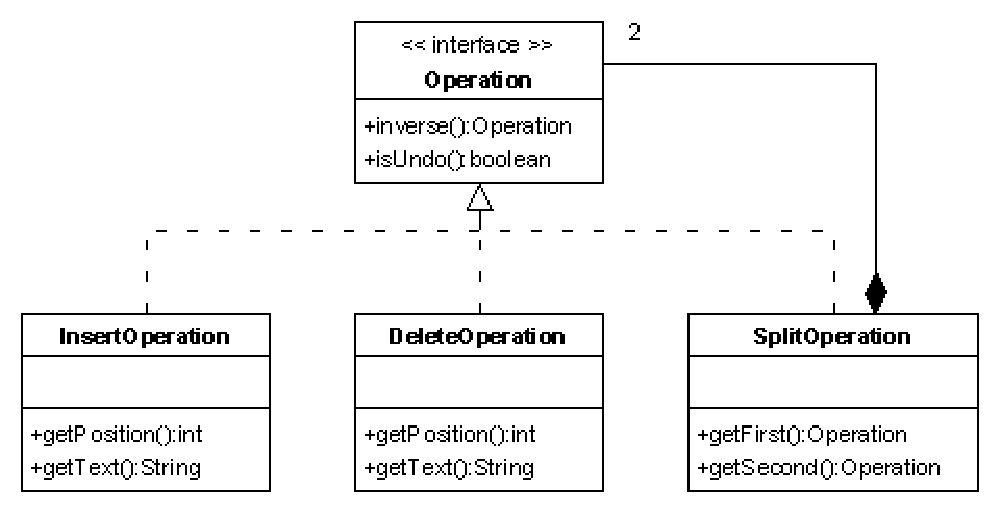
\includegraphics[height=5.74cm,width=11.59cm]{../../images/algo-impl/operation_classdiagram.eps}
\caption{Operation Hierarchy}
\label{Operation Hierarchy}
\end{figure}

\label{Split_Operation}
As depicted in figure \ref{Operation Hierarchy} there exists a third operation besides the \texttt{InsertOperation} and the \texttt{DeleteOperation}. The so-called \texttt{SplitOperation} is a helper object used to encapsulate two delete operations. This is necessary when an insert operation occurs in the range of a delete operation. For more details see \emph{Case 8} in \ref{Delete_Insert}.

\section{Request}
A request is used to distribute changements of a document over the network. It must contain all important informations such as an operation (what has changed and at which position), a timestamp (in which document state this changement has been generated) and a siteID (who has changed it). Figure \ref{Request Class Diagram} shows this relationship.

\begin{figure}[H]
\centering
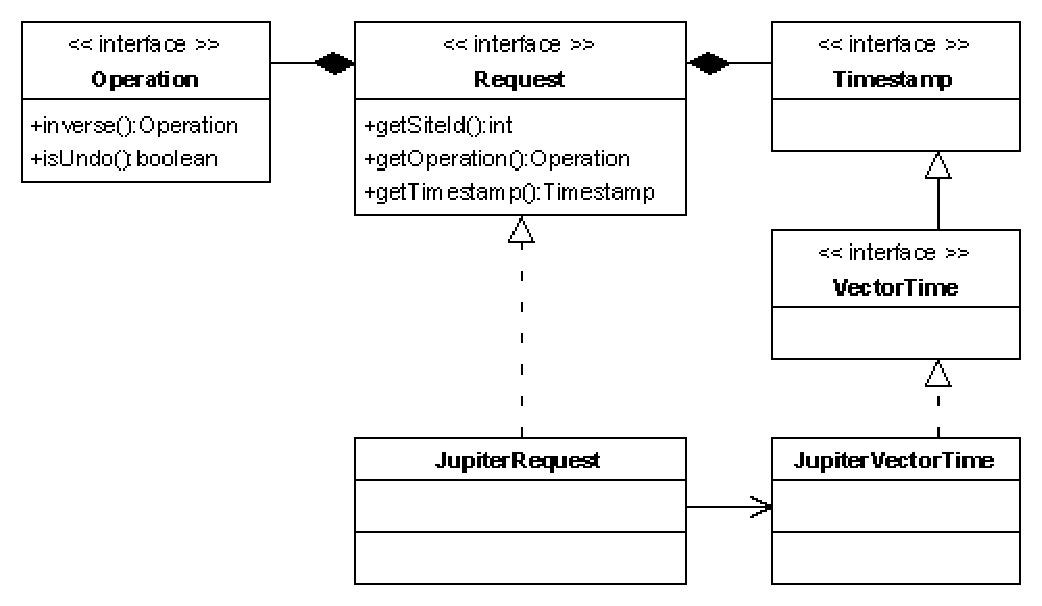
\includegraphics[height=6.87cm,width=12.09cm]{../../images/algo-impl/request_classdiagram.eps}
\caption{Request Class Diagram}
\label{Request Class Diagram}
\end{figure}

How exaclty a request will be send to a server or another client is not part of this chapter and depends on the network technology (see \emph{Report Evaluation Network}) used.


\section{GOTO Transformation Functions}

\subsection{Overview}
The GOTO (generic operation transformation optimized) transformation functions are designed to work with string as well as characters. The advantage is that less transformations are needed when a string has been inserted into a text. To understand the exigence of transformation functions see \emph{Report Evaluation Algorithms}.

The inclusion transformation functions are used to check the influence of a given operation B to another operation A. If so, the operation A will be transformed into operation A'. To transform an operation means to adapt position and text of the operation. In the majority of cases this is a very simple process. But sometimes it is necessary to extract a text fragment or to split up an operation in two parts. For more details about splitting operations into two parts see \ref{Split_Operation}.

All possible transformation \emph{cases} with two insert/delete operations are depicted in figure \ref{Transformation Overview} and explained in the following sections:
\begin{figure}[H]
\centering
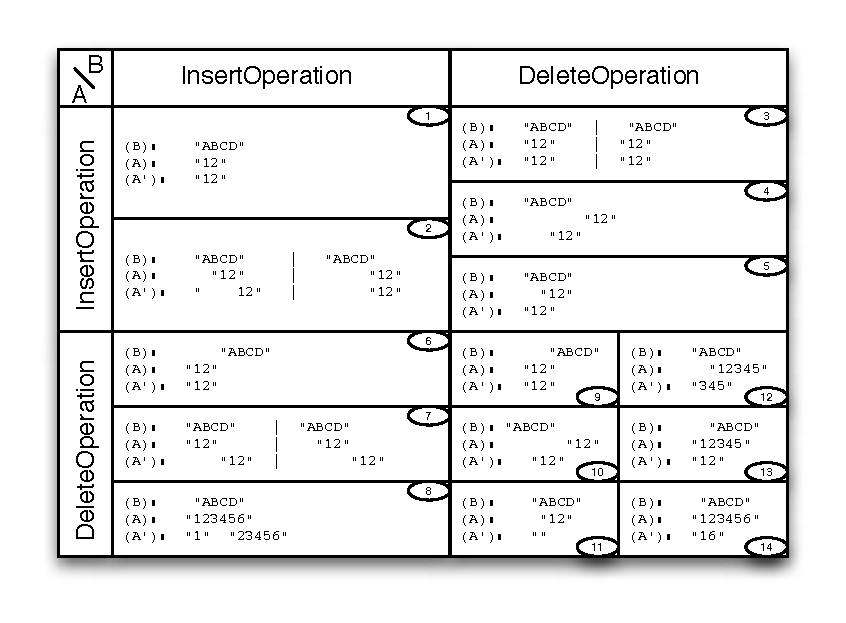
\includegraphics[height=9.98cm,width=13.75cm]{../../images/algo-impl/transform_overview.eps}
\caption{Transformation Overview}
\label{Transformation Overview}
\end{figure}

\subsection{Insert/Insert}
\begin{itemize}
\item \textbf{Case 1:}
Operation A starts before or at the same position as operation B. Sometimes a special handling is necessary. See \emph{Special Case} in section \ref{Special_Case} for detailed information about that.
\item \textbf{Case 2:}
Operation A starts inside or after operation B. Index of operation A' must be increased by the length of the text of operation B.
\item \textbf{Special case:}
\label{Special_Case}
It can occur that two insert operations (for example \texttt{Ins(0,'a')} and \texttt{Ins(0,'b')}) have the same position. How should the correct transformation look like (does the insertion of 'a' have to be before or after 'b')? This is an undecidable problem. Therefore some extra rules must be defined. The first approach to solve this problem is by preferring the operation with the lower ascii value. With this method the final text would be \texttt{ab}. The following figure demonstrates that this solution can violate the user's intention:
\begin{figure}[H]
\centering
%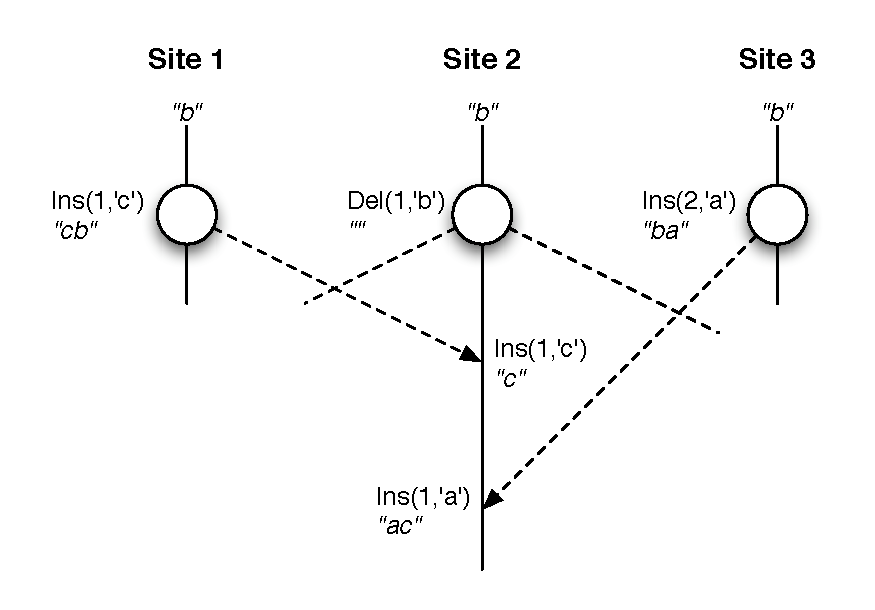
\includegraphics[height=9.77cm,width=14.25cm]{../../images/algo-impl/transform_ins_ins_charpos.eps}
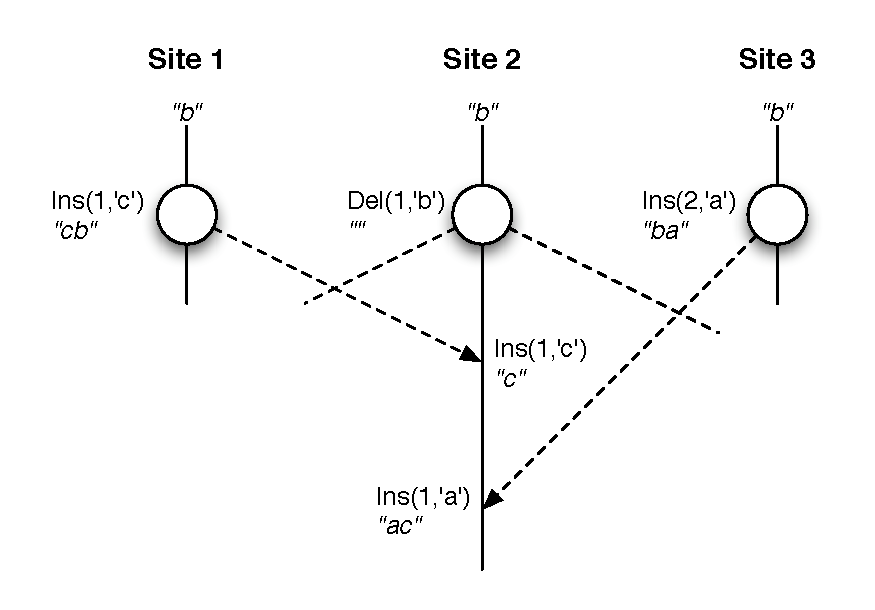
\includegraphics[height=4.63cm,width=7.12cm]{../../images/algo-impl/transform_ins_ins_charpos.eps}
\caption{Transformation based on character code}
\label{Transformation based on character code}
\end{figure}
The scenario depicted in figure \ref{Transformation based on character code} demonstrates an editing session with 3 users (sites). Each site generates a request concurrently. For simplicity only the process flow at site 2 is shown. The initial document state is \texttt{b}. After applying the own operation (\texttt{Del(0,'b')}) then document becomes empty. Then the two other operations arrive. First the operation \texttt{Ins(0,'c')} from site 1 and then \texttt{Ins(1,'a')} from site 3 which will be transformed into \texttt{Ins(0,'a')} because the delete operation has an effect on it. The two operations (\texttt{Ins(0,'a')} and \texttt{Ins(0,'c')}) left remain to be transformed and the problem described in the previous paragraph occures.

The second approach works with some extra information. If an operation has been generated the original position is saved too. Adapted to the scenario in figure \ref{Transformation based on character code} the insert operation of site 1 would look like \texttt{Ins(0,'a',0)}. Similar to the insert operation of site 1 the insert operation of site 3 looks like \texttt{Ins(1,'b',1)}. The added third parameter represents the original position. At the beginning the position and the original position have the same value. The difference of the two positions is shown after a transfomation. Unlike the position (first parameter) the original position will never be transformed/changed and remains the same for the livetime of the operation.

Considering the second approach, the site 1 sends the request \texttt{Ins(0,'c',0)} to site 2. After site 2 received the request, site 3 sends the request \texttt{Ins(1,'a',1)}. On site 2 this request will first be transformed against \texttt{Del(0,'b')} into \texttt{Ins(0,'a',1)}. This is necessary because while site 3 was generating the request, site 2 deleted the character \texttt{b}. After this transformation the new request has to be transformed with the request from site 1. This transformation would look like \texttt{transform( Ins(0,'a',1), Ins(0,'c',0) )} which means that the effect from the operation \texttt{Ins(0,'c',0)}) will be included into operation \texttt{Ins(0,'a',1)}. The problem to solve now is the same as before, but with the extra information its not longer infeasible. After detecting that the two operations have the same position the transformation function compares the original positions. With this solution the \texttt{c} will be inserted before the \texttt{a} and the user intention is preserved.

Figure \ref{Transformation based on character code} shows that even with using original positions another problem can occur:
\begin{figure}[H]
\centering
%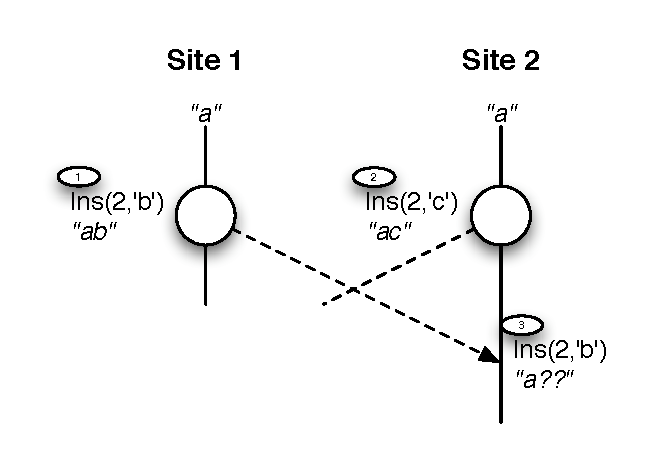
\includegraphics[height=7.26cm,width=10.26cm]{../../images/algo-impl/transform_ins_ins_origpos.eps}
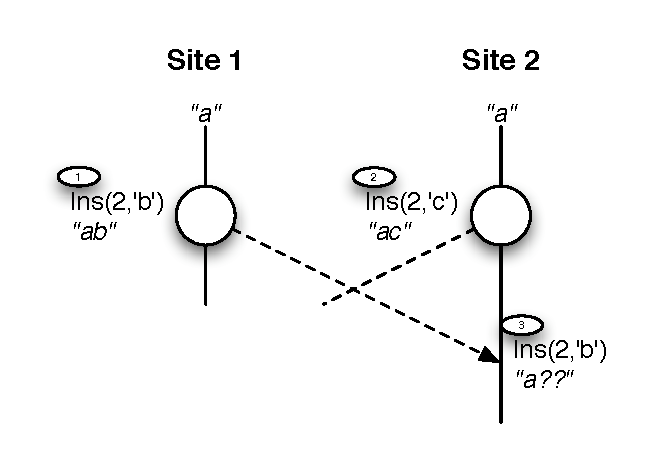
\includegraphics[height=3.63cm,width=5.13cm]{../../images/algo-impl/transform_ins_ins_origpos.eps}
\caption{Transformation based on equal original positions}
\label{Transformation based on equal original positions}
\end{figure}
At the same time each site generates an insert operation with the same position. The insert operation from site 1 looks like \texttt{Ins(1,'b',1)} and the operation from site 2 is \texttt{Ins(1,'c',1)}. When site 2 receives the request from site 1 the operations have to be tranformed (\texttt{transform( Ins(1,'b',1) , Ins(1,'c',1) )}). The transformation function will detect that the two operations have the same position and will check the original positions. Unfortunately the original positions have the same values. Therefore the approach to solve this problem by using original positions will fail too.

This problem can only be eliminated by privileging one operation. But which operation should be preferred? And how to guarantee that on all sites this will be the same operation? One possible solution would be to use the site id's (e.g. site 1 is always privileged against site 2 and site 3, site 2 is only to site 3). Especially when using this transformation functions with the \emph{Jupiter} algorithm, the operation which has been issued by the server side is always privileged (client/server flag).

\item \textbf{LSP:}
TODO

\end{itemize}

\subsection{Insert/Delete}
\begin{itemize}
\item \textbf{Case 3:}
Operation A starts before or at the same position as operation B. Nothing has to be transformed.
\item \textbf{Case 4:}
Operation A starts after operation B. Index of operation A' must be reduced by the length of the text of operation B.
\item \textbf{Case 5:}
Operation A starts inside operation B. Index of operation A' must be the index of operation B.
\end{itemize}

\subsection{Delete/Insert}
\label{Delete_Insert}
\begin{itemize}
\item \textbf{Case 6:}
Operation A is completly before operation B. Nothing has to be transformed.
\item \textbf{Case 7:}
Operation A starts before or at the same position as operation B. Index of operation A' must be increased by the length of the text of operation B.
\item \textbf{Case 8:}
Operation B is in the range of operation A. Operation A' must be splitted into two delete operations. For more details about the split operation see \ref{Split_Operation}.
\end{itemize}

\subsection{Delete/Delete}
\begin{itemize}
\item \textbf{Case 9:}
Operation A is completely before operation B. Nothing has to be transformed.
\item \textbf{Case 10:}
Operation A starts at the end or after operation B. Index of operation A' must be reduced by the length of the text of operation B.
\item \textbf{Case 11:}
Operation A and operation B are overlapping. Operation B starts before or at the same position as operation A and ends after or at the same position as operation A. Content of operation A has already been deleted by operation B. Therefore, nothing has to be deleted anymore by operation A. A' is called a noop (no-operation).
\item \textbf{Case 12:}
Operation A and operation B are overlapping. Operation B starts before or at the same position as operation A and ends before operation A. The overlapping part of the two operations has been deleted by operation B. Operation A' has to delete only the remaining text (text after the overlapping text of the two operations).
\item \textbf{Case 13:}
Operation A and operation B are overlapping. Operation B starts after operation A and ends after or at the same position as operation A. The overlapping part of the two operations has been deleted by operation B. Operation A' has to delete the remaining text (text before the overlapping text of the two operations).
\item \textbf{Case 14:}
Operation A and operation B are overlapping. Operation B inside fully in operation A. The overlapping part of the two operations has been deleted by operation B. Operation A' has to delete the remaining text (text before and after the overlapping text of the two operations).
\end{itemize}


\section{Algorithm}
\begin{figure}[H]
\centering
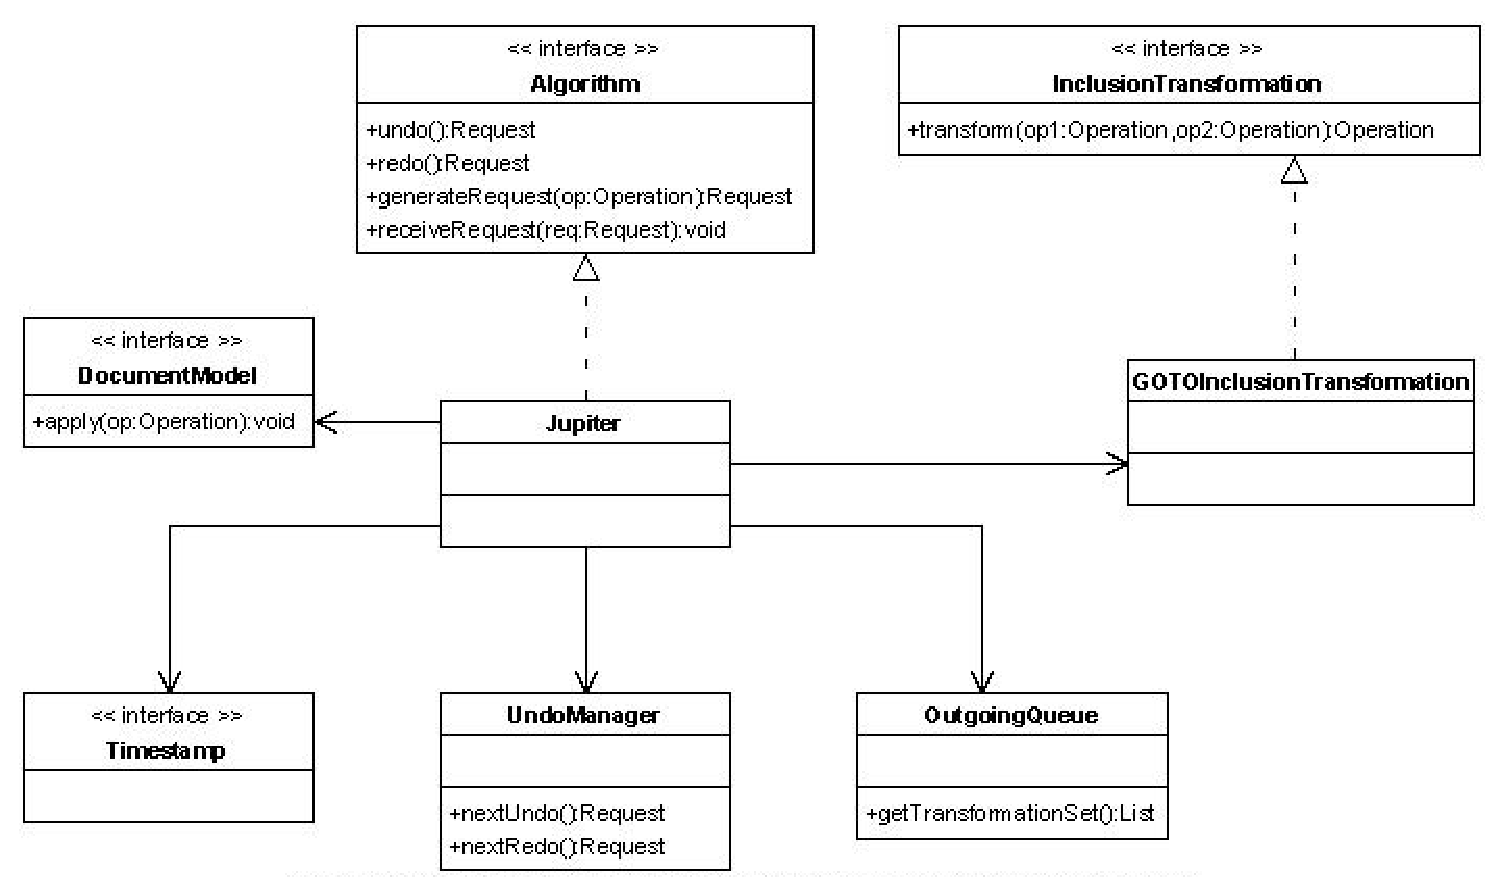
\includegraphics[height=8.74cm,width=14.95cm]{../../images/algo-impl/algorithm_diagram.eps}
\caption{Algorithm architecture}
\label{Algorithm architecture}
\end{figure}

The algorithm component centers around the Jupiter class, which is an implementation of the Algorithm interface. Jupiter processes all requests with the collaboration of the GOTOInclusionTransformation. All transformed operations are applied to the DocumentModel instance. The Timestamp class represents the current state vector, i.e. the location in the 2-dimensional state space of the \emph{Jupiter} algorithm. The UndoManager class is apparently used for undo/redo functionality and is further described in \ref{undo_redo}.


\section{Client}
\begin{figure}[H]
\centering
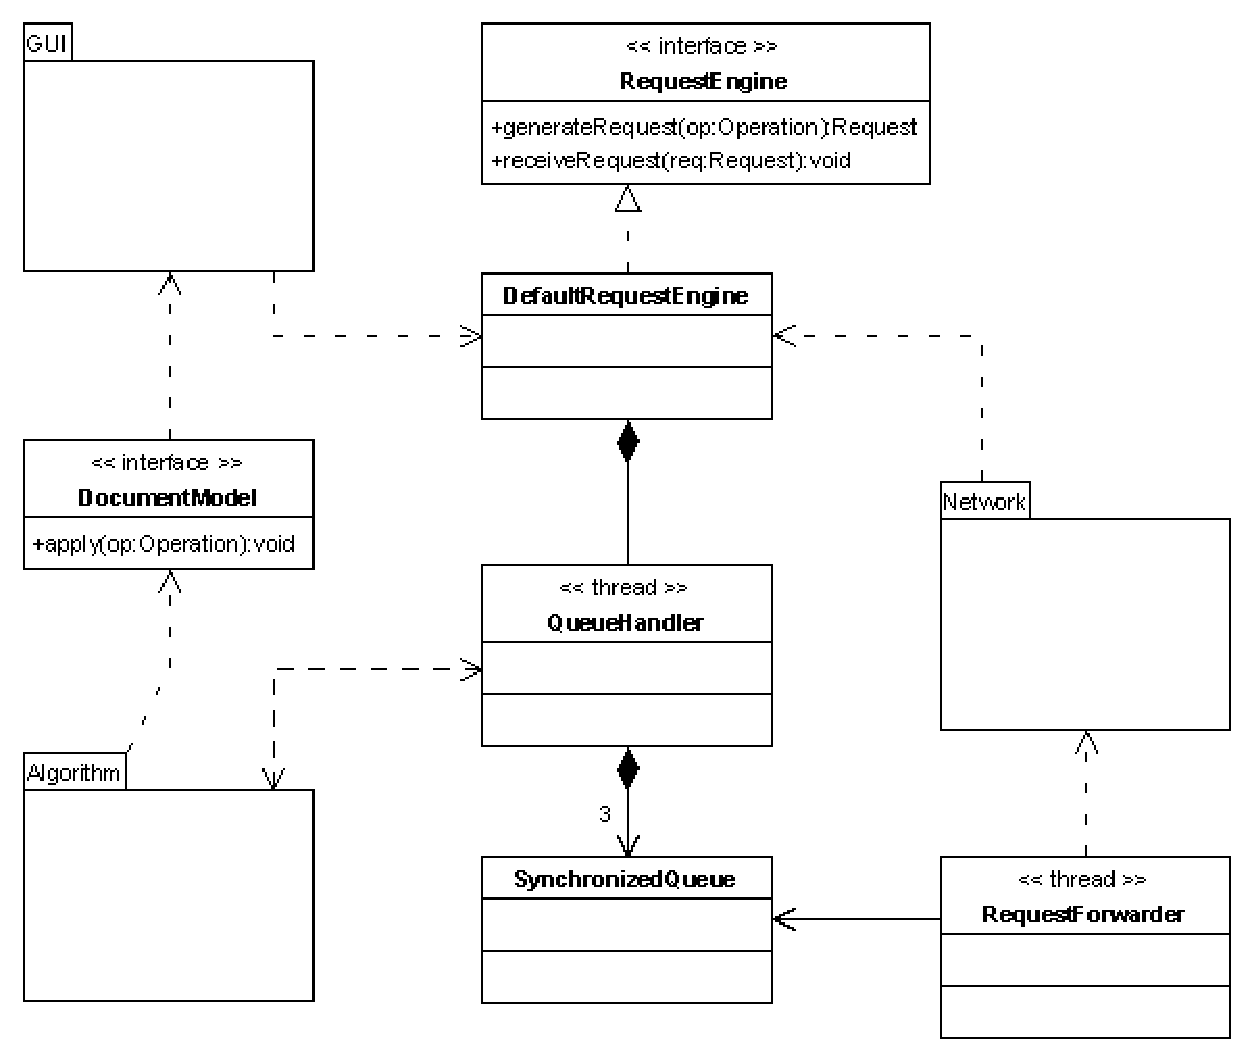
\includegraphics[height=13.04cm,width=15.46cm]{../../images/algo-impl/client_diagram.eps}
\caption{Client architecture}
\label{Client architecture}
\end{figure}

The client component centers around the RequestEngine class. The RequestEngine is a mediator between the GUI, network and algorithm components. It receives requests from the GUI and the network, respectively. All requests are passed to synchronized queues, one for local requests and one for remote requests. The requests are read out from the queues by the QueueHandler class. This thread waits on the queues until a request has been received. Each request is then handed to the algorithm package for processing. Processing involves transforming the operation and applying it to the document model. 

Locally generated requests are returned from the algorithm package  to the QueueHandler which in turn passes it to another SynchronizedQueue, namely the outgoing queue. From there, all outgoing requests are forwarded to the network package by the RequestForwarder class. 


\section{Server}
\begin{figure}[H]
\centering
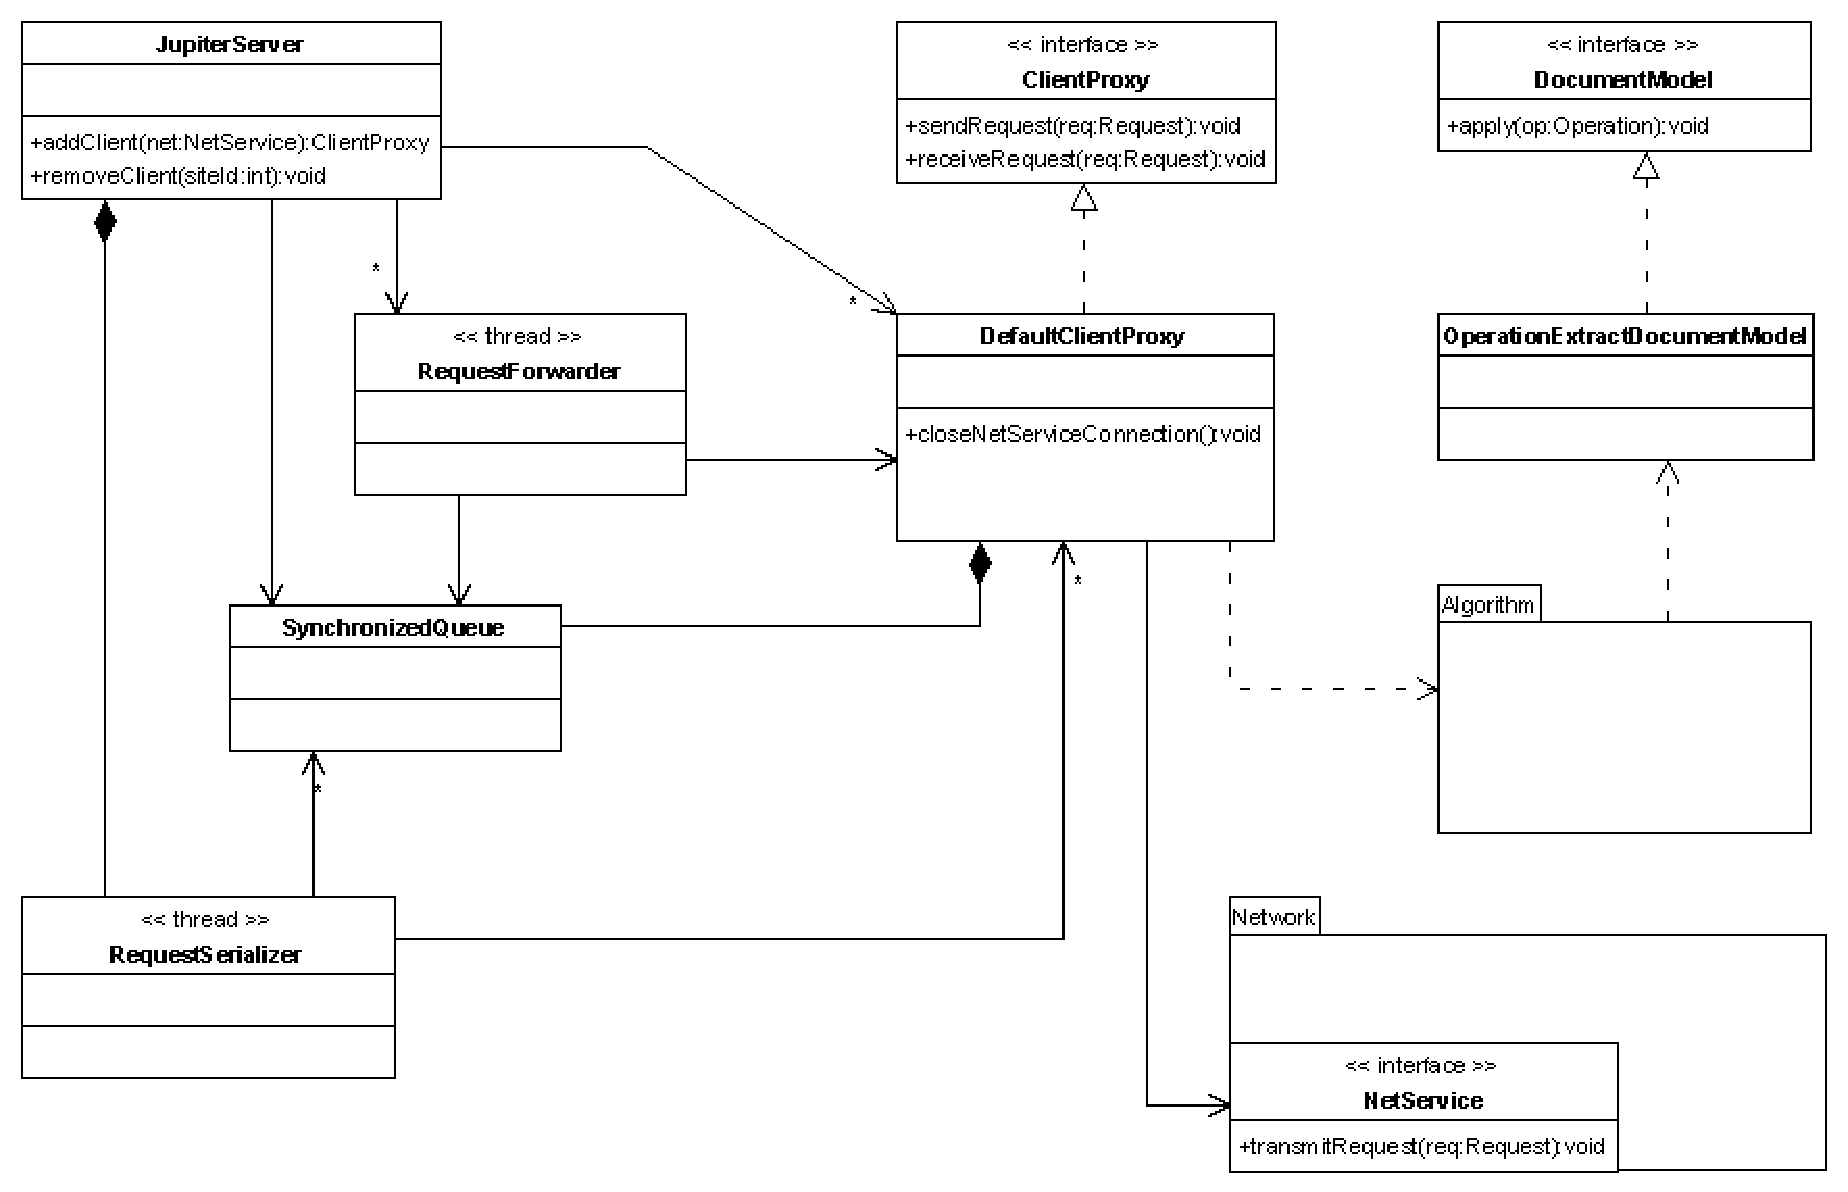
\includegraphics[height=9.8cm,width=15.36cm]{../../images/algo-impl/server_diagram.eps}
\caption{Server architecture}
\label{Server architecture}
\end{figure}

The \emph{Jupiter} server component is the turntable in a multi-user collaborative editing session. It achieves n-way communication by use of the 2-way synchronization protocol of \emph{Jupiter} between each client and its corresponding ClientProxy on the server side (instances of class ClientProxy). The \emph{Jupiter} server component can be started and organized by creating a new instance of class JupiterServer. It allows to manage client proxies, that is to add and remove them.

\subsection{Adding a client}
When a new client is added to the server, a new ClientProxy is created. It is passed references to instances of the following types: NetService, Algorithm (Jupiter), SynchronizedQueue. The NetService class is used to forward outgoing requests to the network layer. The algorithm is responsible for the operational transformation. Since no real document model is used at the server side, a special implementation of the DocumentModel interface, OperationExtractDocumentModel, lets the algorithm extract the latest applied operation.

Afterwards, the ClientProxy instance is added to the RequestSerializer. Finally, a RequestForwarder for this ClientProxy is created. It is responsible for forwarding all requests that were issued by other clients and are to be sent to the opposite of the ClientProxy, namely the client itself. The RequestForwarder reads requests from the SynchronizedQueue and passes them to the ClientProxy by invoking $sendRequest(request)$.

\subsection{Removing a client}
When a client proxy is to be removed, firstly its connection to the net service is closed. Then the RequestForwarder, belonging to the client proxy, is shut down. Finally, the client proxy is removed from the RequestSerializer. The removal from the RequestSerializer is more complicated. At the time of removal, there may still be a couple of requests which have been issued by the client to be removed. Therefore, the client proxy may not be removed until all these requests have been processed, i.e. transformed and sent to all other clients. This is done by remembering the number of requests in the request queue, say $r$. After $r$ requests have been processed from that moment on, the client proxy can savely be released. This mechanism is achieved by a helper class named Counter.

\subsection{Receiving and sending a request}
The received request is passed from the network layer to the corresponding ClientProxy instance. The ClientProxy itself only forwards the request to the SynchronizedQueue, namely request queue. Actually all ClientProxy's forward their requests to the same synchronized queue. By that, a global serialization is achieved. From the request queue, the request is read out by the RequestSerializer thread. The request is then passed to its corresponding client proxy for transformation. Afterwards, the transformed request is distributed to all other clients. This is done by first calling $generateRequest(operation)$ on each ClientProxy's algorithm and then adding the returned request to the outgoing queue of the ClientProxy. From there, the RequestForwarder will read out the request and pass it to the ClientProxy which in turn forwards it to the net service. Finally, the net service transmits the request to the client.

The SynchronizedQueue's enable us to have a flexible interaction of the different components such as ClientProxy, RequestSerializer, RequestForwarder. No component blocks except the ones which read from the queue, e.g. RequestSerializer, RequestForwarder.

\section{Undo/Redo}
\label{undo_redo}
For the undo implementation, we worked closely with the paper "Reducing the Problems of Group Undo" from Ressel et al., adapting the \emph{adOPTed} undo for the \emph{Jupiter} algorithm. 
The implementation of undo functionality has started but has not finished by the time. The undo works in simple cases both for characterwise and stringwise operations. But it fails in more complex scenarios (cf. classes $JupiterCharUndoTest.java$ and $JupiterStringUndoTest.java$, respectively. At first, we assumed that we could implement the undo with some auxiliary data structures and would not have to build the whole state space. In fact, it worked for example 3 as well as for example 4 (known as the "del-del-undo-puzzle") taken from the above paper, but it finally failed at the "order puzzle" in figure 6 of the same paper. The "order puzzle" showed us that the auxiliary data structures would not be sufficient for more complex undo scenarios and that we would need to implement the whole state space as is the case in the \emph{adOPTed} algorithm and undo, respectively. 
Therefore we will not further describe the undo implementation we have done so far as much of it will become unusable as soon as we implement the state space. Building the state space means keeping track of every operation and calculating all possible transformation paths.

Nevertheless, two issues will remain. Firstly, each operation has a method $isUndo()$ to detect undo operations and to treat them separately. Secondly, the UndoManager class is used to manage undo and redo requests.

\section{Tests}
Testing the algorithm implementation was considered a very high priority. Without a correctly working algorithm, it will be difficult or even impossible to create a collaborative text-editor. Because of the significance of this algorithm we invested a lot of time to test it.

\subsection{Testframework}
In the literature about operational transformation, so called puzzles are omnipresent. These puzzles are exact specification of the order of events, like the generation of a request or the reception of a request. We were soon convinced that in order to test our algorithm it would be possible to have a testframework that accepts such a puzzle (called scenario) as input and replays the sequence of events on a set of algorithms. To find out more about this testframework, see the document emph{Report Implementation Testframework}.

\subsection{Test Cases}
We gathered many test cases form publications about operational transformation algorithms. The puzzles presented in these papers often represent particularly tricky issues that other algorithms failed to resolve. Here is a list of test cases that were taken from papers:

% TODO: insert all test cases that were taken from papers
\begin{itemize}
 \item Figures 3, 4 and 5 in "Proving Correctness of Transformation Functions in Real-Time Groupware", Imine et al.
 \item "C2 puzzle P1" and "C2 puzzle P2" (figures 3 and 5, respectively) in "Achieving Convergence with Operational Transformation in Distributed Groupware Systems", Imine et al.
 \item "A scenario of divergence and ERV" and  "A divergence and ERV scenario of IMOR" (figures 1 and 12, respectively) in "Preserving Operation Effects Relation in Group Editors", Du Li and Rui Li
 \item figure 5 in "Concurrent Operations in a Distributed and Mobile Collaborative Environment", Suleiman et al.
 \item the "dOPT puzzle" (figure 2) in "Operational Transformation in Real-Time Group Editors: Issues, Algorithms, Achievements", Sun et al. 
\end{itemize}

Our algorithm is capable of solving these complex puzzles. This is a step in the right direction, but that alone is not enough. So we devised additional test cases that cover trivial as well as complex scenarios.

\subsection{JUnit Tests}
It is one of our goals to have a good test coverage with \emph{JUnit} tests.
